\section{Experimental Results}
The proposed system has been evaluated on five synthetic and six real
datasets. All the experiments have been performed on an Intel Core i7-4770
($3.40$GHz, single thread) machine with $32.0$GB RAM. MATLAB with some
C++ mex functions are used for the implementation.

\mysubsubsection{Synthetic data} We generate synthetic indoor 3D models
as shown in~\Fref{fig:synth}.
%
\begin{figure}[!t]
\begin{center}
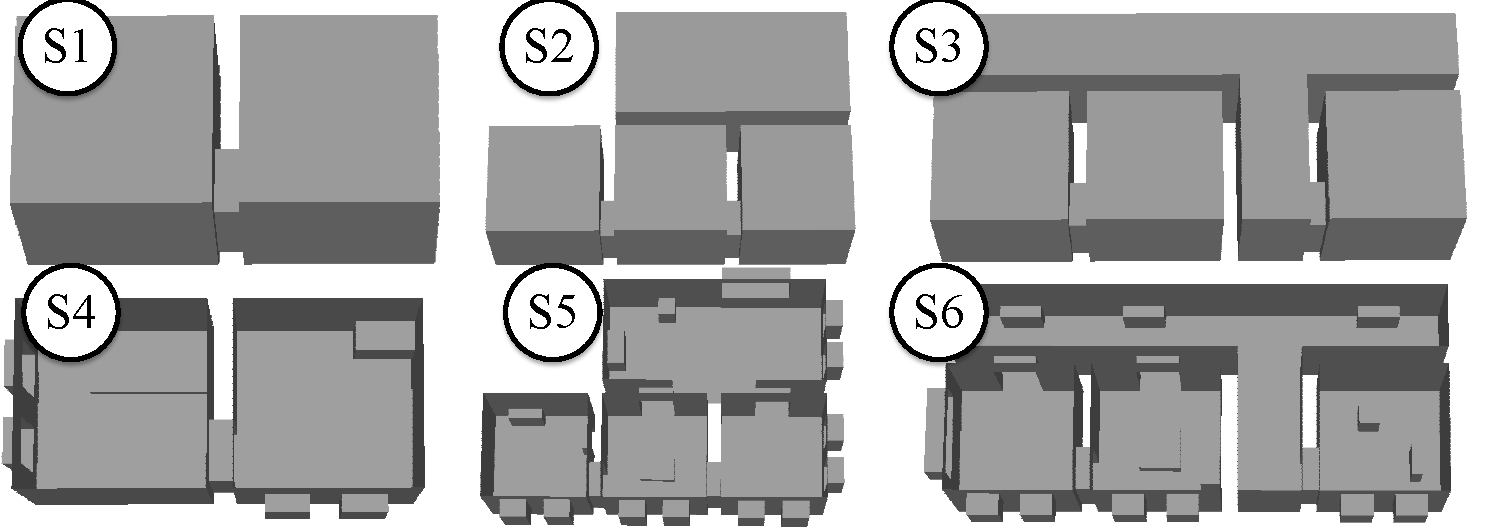
\includegraphics[width=85mm]{../figures/synth2.pdf}
\end{center}
 \vspace{-0.3cm}
\caption{Synthetic datasets. RGB-D panoramas are generated from sparsely
distributed viewpoints from these meshes.}  \label{fig:synth}
 \vspace{-0.2cm}
\end{figure}
%
The first three datasets (S1)-(S3) contain multiple rooms ($2$ or $4$)
but without any details on the walls, floors or ceilings. The latter
three datasets (S4)-(S5) have the same rooms but also contain objects
and wall details.

We compare our algorithm against the baseline methods in Computer
Graphics and Computer Vision, namely, the screened poisson
reconstruction algorithm (Poission)~\cite{Kazhdan2013} and the Manhattan
volumetric graphcuts algorithm (Vgcuts)~\cite{furukawa-iccv-2009}. We
are interested in the trade-off between the geometric accuracy and the
model complexity (\eg., the number of polygons in the model). Therefore,
a standard mesh simplification algorithm~\cite{Tarini2010} is used to
control the numbers of polygons for Poisson. For Vgcuts, we tune the
weight on the smoothness penalty to control the polygon counts. For both
methods, we generated a low-res and high-res mesh models. The polygon
count of the low-res model is set to be very close to ours. Each mesh
model is rasterized into a panorama image to generate a depth image
together with the surface normal information.

The positional and the normal accuracies are measured simply by the
average error from the ground truth over the rasterized pixels
(See~\Tref{table:quantitative}). Note that even without the object
point clouds, our method achieves high precision thanks to the our compact but accurate detail reconstruction algorithm. 
%Note that our mesh model conveys useful structural information, while
%other methods simply produce a polygon soup, whose applications are
%limited.
Errors are mainly due to the lack of objects, which can be verified by
our results with object point clouds, which are also rasterized with
splatting for evaluation.  Vgcuts has a strong axis-aligned
regularization, and tends to lose details due to the shrinkage bias.
\begin{table}[!t]
\caption{Positional [mm] and normal errors [degrees] (inside
 parentheses) on synthetic data.}
\begin{center}
 \vspace{-0.5cm} 
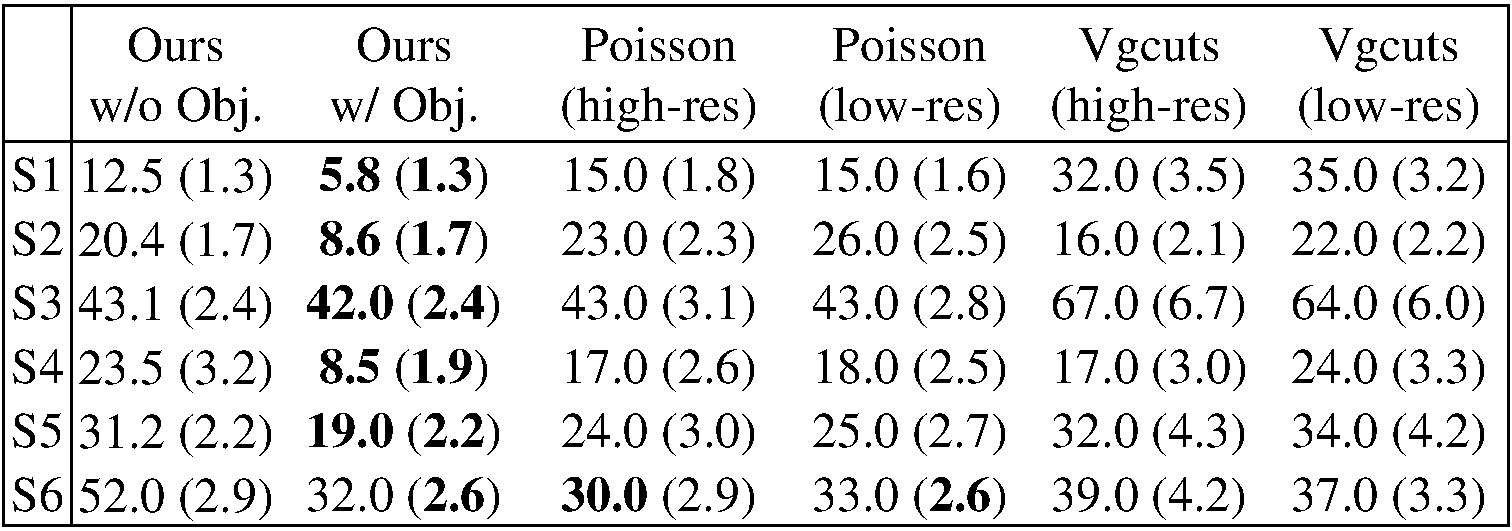
\includegraphics[width=85mm]{../figures/quantitative.pdf}
\end{center}
\label{table:quantitative}
 \vspace{-0.3cm}
\end{table}


%
% simplification algorithm, and the resultant mesh
% complexity of~\cite{furukawa-iccv-2009} by changing the smoothness
% parameter of the potts cost ($\lambda = 8,4,2$).
%
% The results are illustrated in. Here the number of meshes of Poission is
% reduced to $10000$, $1000$, and exactly the same number of our mesh
% % model. In totally, we observe that our method outperforms other
% algorithms in almost all datasets for the accuracy and model
% complexity. Interestingly, our model works mostly better than the
% poisson surface reconstructions that finds the implicit surfaces of the
% input noise-less point cloud since our method could recover the surface
% where the point cloud is very sparse due to occlusions. We observe that
% the VGCuts algorithm suffered from the shrinkage bias and destroyed many
% thin wall structures.



\mysubsubsection{Real data}
Figure~\ref{fig:result_real} illustrates the five real datasets, where
their statistics are summarized in~\Tref{table:statistics}.
\begin{figure*}[!t]
\begin{center}
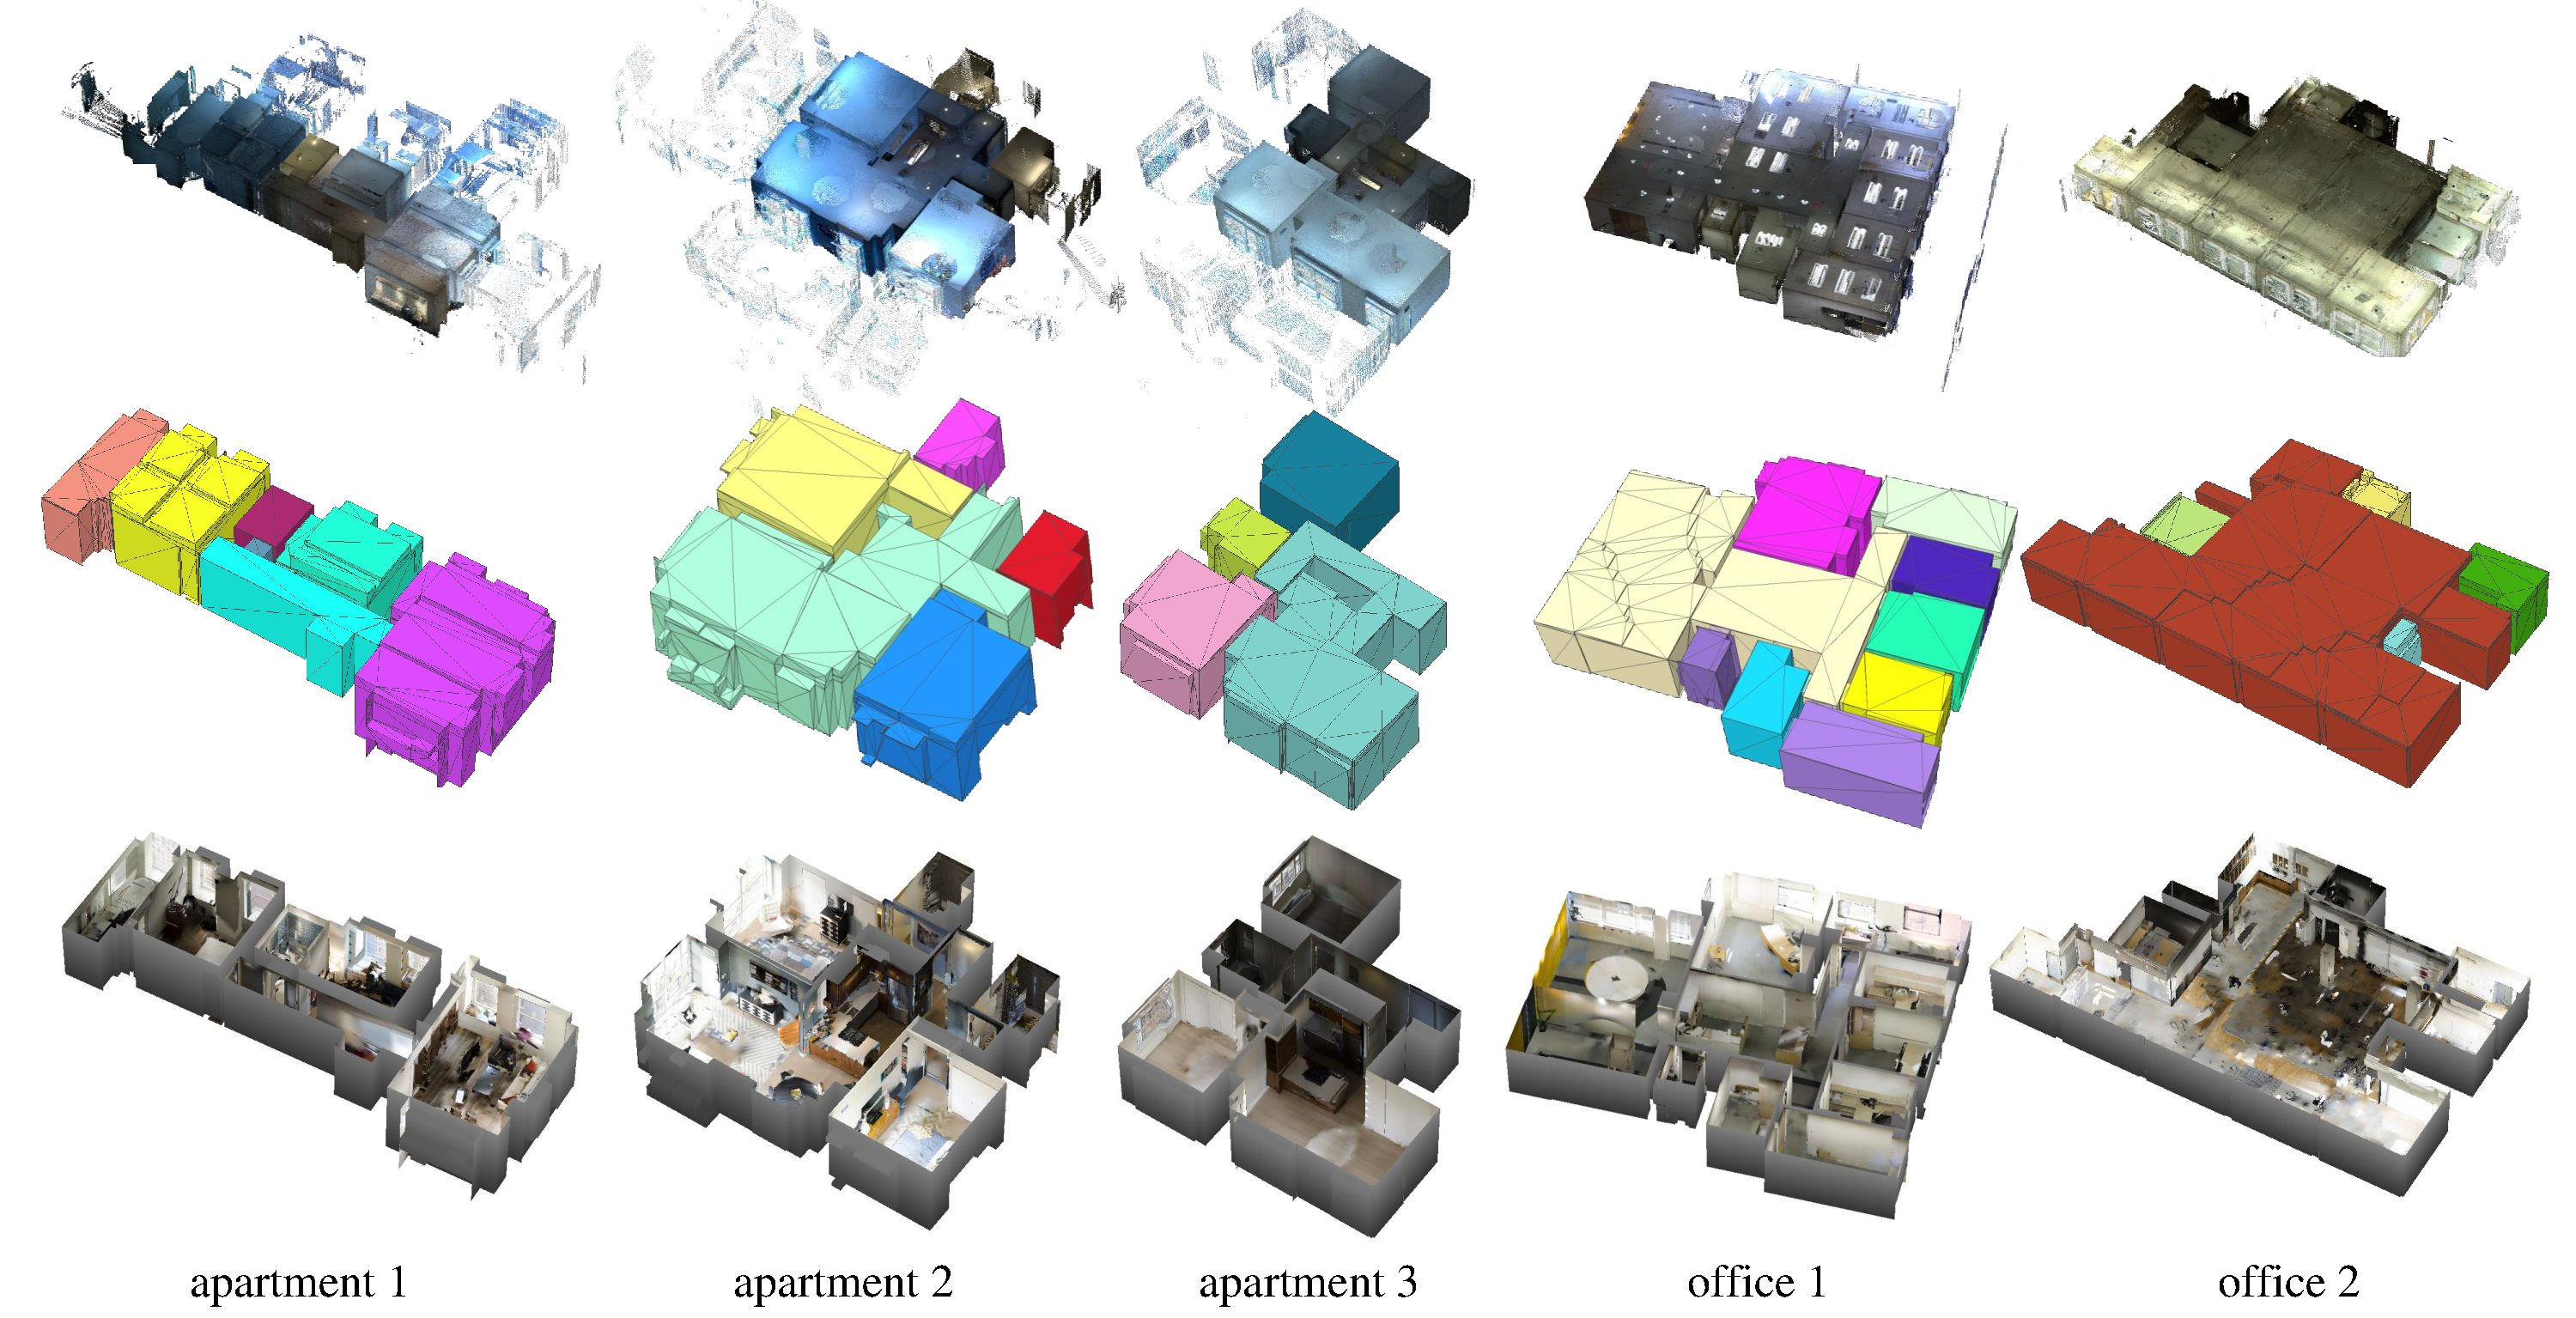
\includegraphics[width=150mm]{../figures/result_real.pdf}
\end{center}
 \vspace{-0.3cm}
\caption{Results on the real datasets.  From top to bottom: the input
 point clouds, the reconstructed mesh models, and sample renderings.}
 \label{fig:result_real}
 \vspace{-0.25cm}
\end{figure*}
\begin{table}[!t]
\caption{Statistics of the real experiments. Here we show the number of
 elements reconstructed and the geometric distance from the input depth
 map and reconstructed surface geometry compiled with (a) walls, (b)
 walls+details, (c) walls+details+objects. We also show the
 computational time of the entire pipeline.}
 \vspace{-0.5cm}
\begin{center}
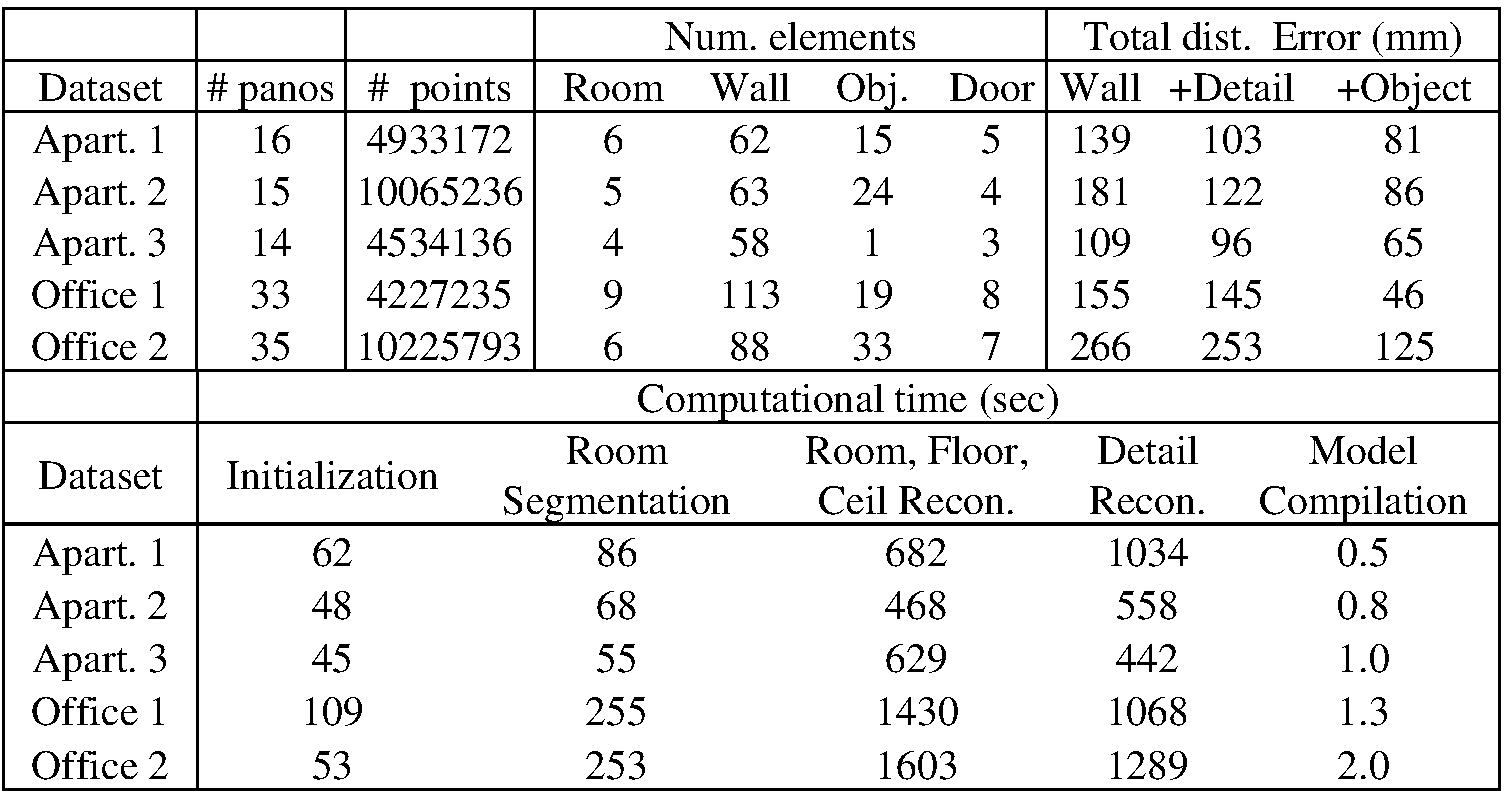
\includegraphics[width=85mm]{../figures/statistics.pdf}
\end{center}
\label{table:statistics}
 \vspace{-0.7cm}
\end{table}
% We also evaluate our algorithm using five real datasets: a set of (1)
% {\it apartment } dataset (16 panoramas), (2) {\it apartment 2} dataset
% (15 panoramas), (3) {\it apartment 3} dataset (14 panoramas), (4) {\it
% office 1} dataset (33 panoramas), and (5) {\it office 2} dataset (35
% panoramas). \footnote{The number of points or examples of actual
% panorama images are shown in the supplementary.}
Unlike the synthetic datasets, 3D points in the real datasets are corrupted by
mirrors, windows, reflective objects, and calibration errors.
%
%
The second row in Fig.~\ref{fig:result_real} shows the reconstructed
meshes, compiled from the leaf nodes except for objects in the
structure graph. The color of each geometry is determined by the
parent room node. The third row shows the full renderings including the
object point clouds, which are rendered by the point-based rendering
technique. Note that ceiling geometries are not rendered on purpose to
visualize the interior, which is not easy for polygon soup mesh
models.
% More evaluations are provided in the supplementary material.
%
% At the second rows, we show the reconstructed manifold meshes compiled
% with room, wall, floor, ceiling, and their children details excluding
% the objects node (room segmentation is illustrated by color).
%At the third rows, the texture mapped models compiled with object nodes
%are illustrated. Since we do not have ground truth surfaces, it is quite
%hard to quantitatively evaluate these results, however
%We can qualitatively judge the quality of the results
%by examining the texture-mapped model at the third rows, since if the
%geometry is incorrect, it gives the unnatural sense when looking at the
%textured model.
%
%
%
Although it is difficult to conduct quantitative evaluations on real
datasets, Table~\ref{table:statistics} provides positional errors (the
same metric as in Table~\ref{table:quantitative}) of our model with and
without the wall details and the object point clouds.
More evaluations including qualitative and quantitative comparisons
against Poisson and Vgcuts meshes are provided in the supplementary material.


% Furthermore, we also give statistics
% of our reconstruction in each major steps. In addition, we give the
% total distance between the reconstructed geometry and input point clouds
% that explains how each configuration fits to the input. It is worth
% noting that while the reconstruction of the structured graph takes time,
% the compilation of the model is quite fast since the mesh/point cloud
% have already been attached to the element and we can immediately output
% the model if the leaf nodes are selected.



% \begin{figure}[!t]
% 	\begin{center}
% 		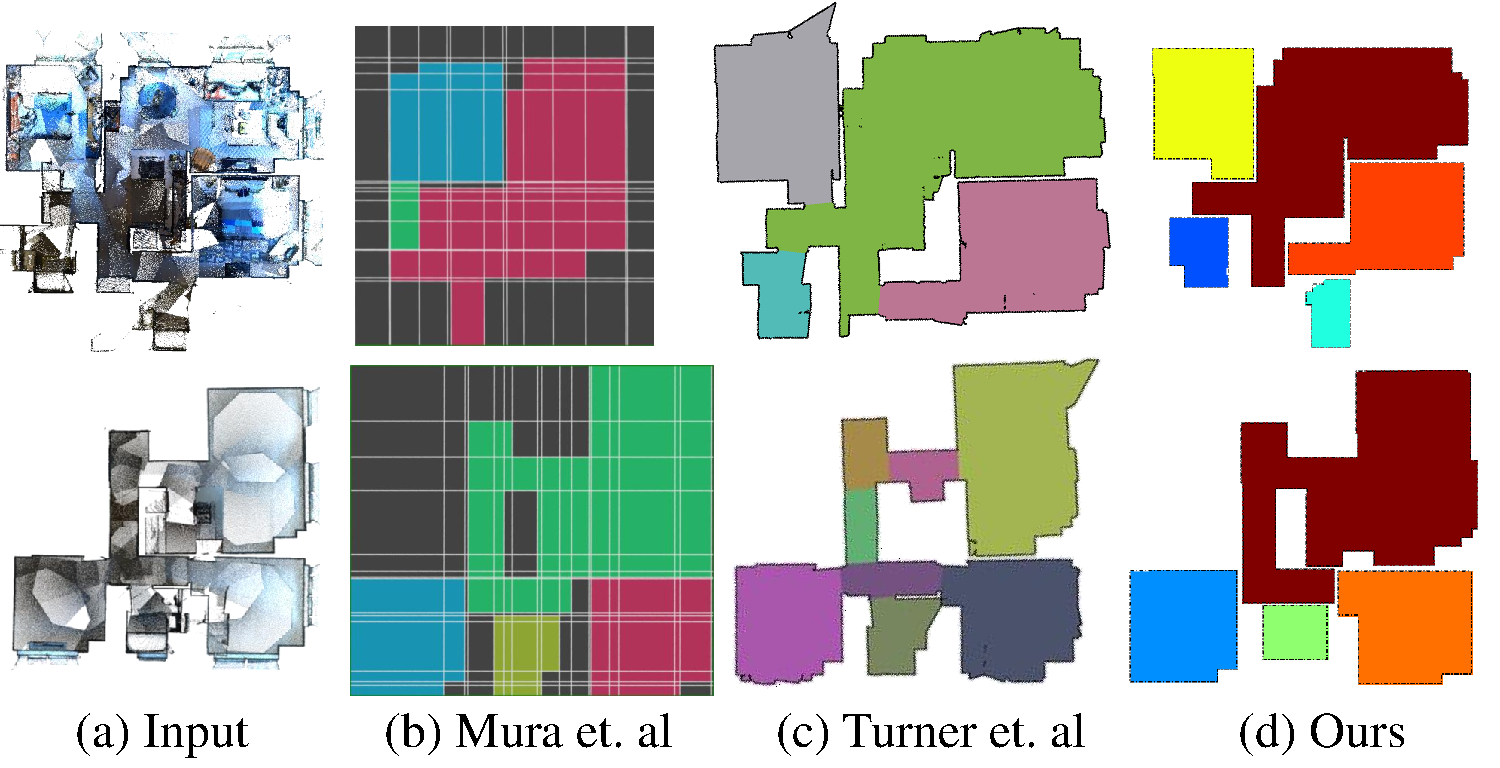
\includegraphics[width=85mm]{../figures/comp_segmentation.pdf}
% 	\end{center}
% 	\caption{\yasu{rotate and flip equal sky from zurich}Comparison of the room segmentation algorithms. Here we show the result of real dataset (a) lumber-cashew, (b) equal-sky, (c) red-lion, (d) new-breeze, and (e) salmon-palace. The first rows are the segmentation result by~\cite{Turner2015}, and the second rows are our room segmentation results. At the third rows, we also show the input point cloud where the points that are higher than camera positions are removed.}
% 	\label{fig:result_berkeley}
% \end{figure}


Figure~\ref{fig:comp_samemesh} qualitatively compares our
reconstructions against Poisson and Vgcuts. Again, the mesh
simplification algorithm~\cite{Tarini2010} and the parameter tuning is
used to make their polygon counts close to ours. The figure shows that
both Poisson and Vgcuts models contain clutters. Instead, our approach
successfully ignores clutters in modeling architectural components,
yielding clean building structure. These clean models enable high
quality texture mapping and rendering experiences, as well as,
interesting post geometry processing.
\begin{figure}[!t]
\begin{center}
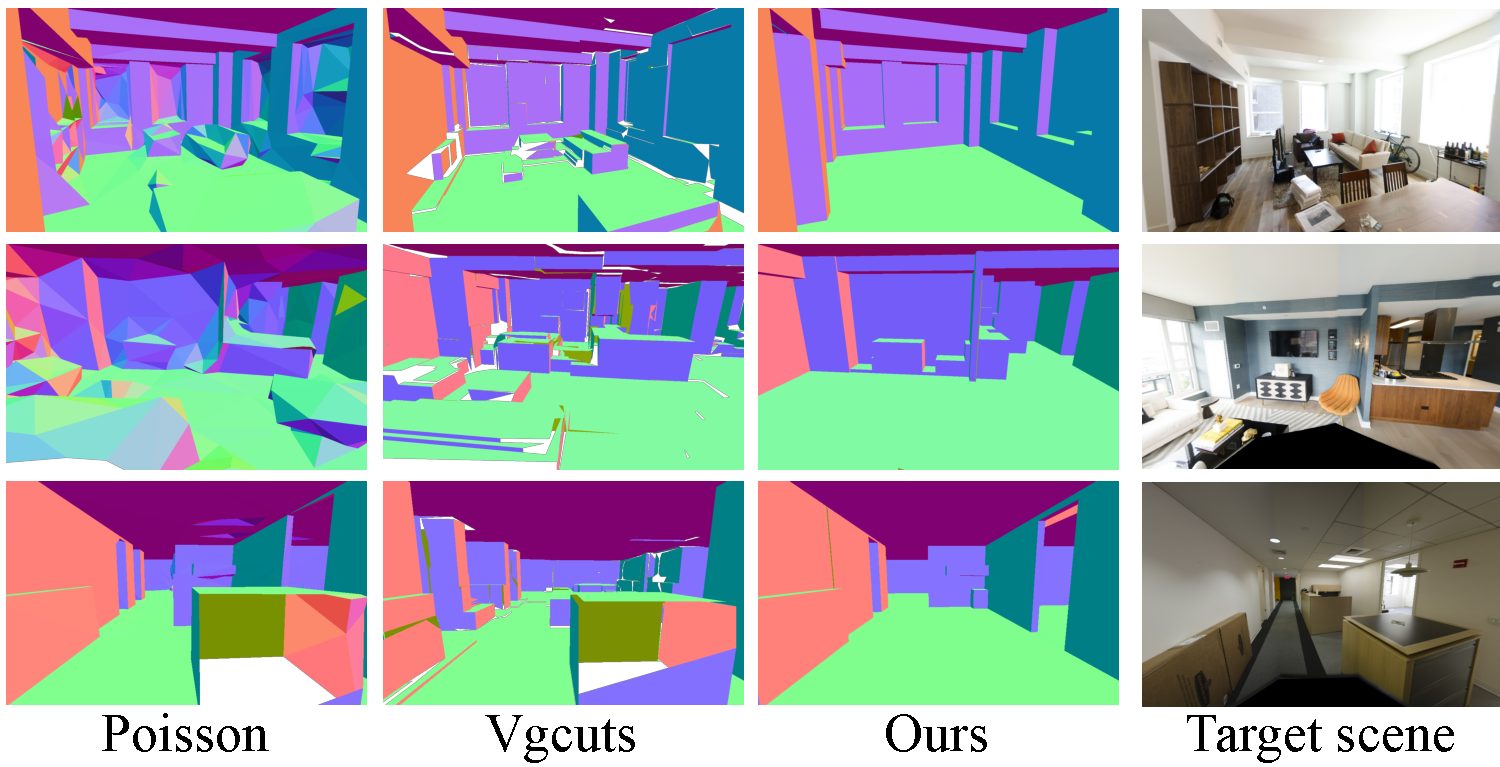
\includegraphics[width=85mm]{../figures/comp_samemesh.pdf}
\end{center}
 \vspace{-0.3cm}
\caption{Comparison with the same number of triangular meshes. Here we show the result of (a)Poisson, (b) Vgcuts, and (c) ours. Note that we simplify the original meshes of Poisson and Vgcuts so that the models contain the same number of polygons with ours.}
\label{fig:comp_samemesh}
 \vspace{-0.25cm}
\end{figure}

We compare our room segmentation process against two state-of-the-art
methods~\cite{Mura2014,Turner2015} in Fig.~\ref{fig:result_all}.  We
asked the authors to process our data. Our method provides reasonable
segmentation that mostly preserves the number of structural cluster
(\eg, room, aisle) and important details.
%, although occasionally produce under-segmented results (\eg, office1).
The over-segmentation is often observed in~\cite{Turner2015}, and the
room shape is too simplified and important details often disappear
in~\cite{Mura2014}. Note that the results could not be obtained for
three datasets by ~\cite{Mura2014}, mainly due to the failures in the
primitive extraction step.
\begin{figure}[!t]
\begin{center}
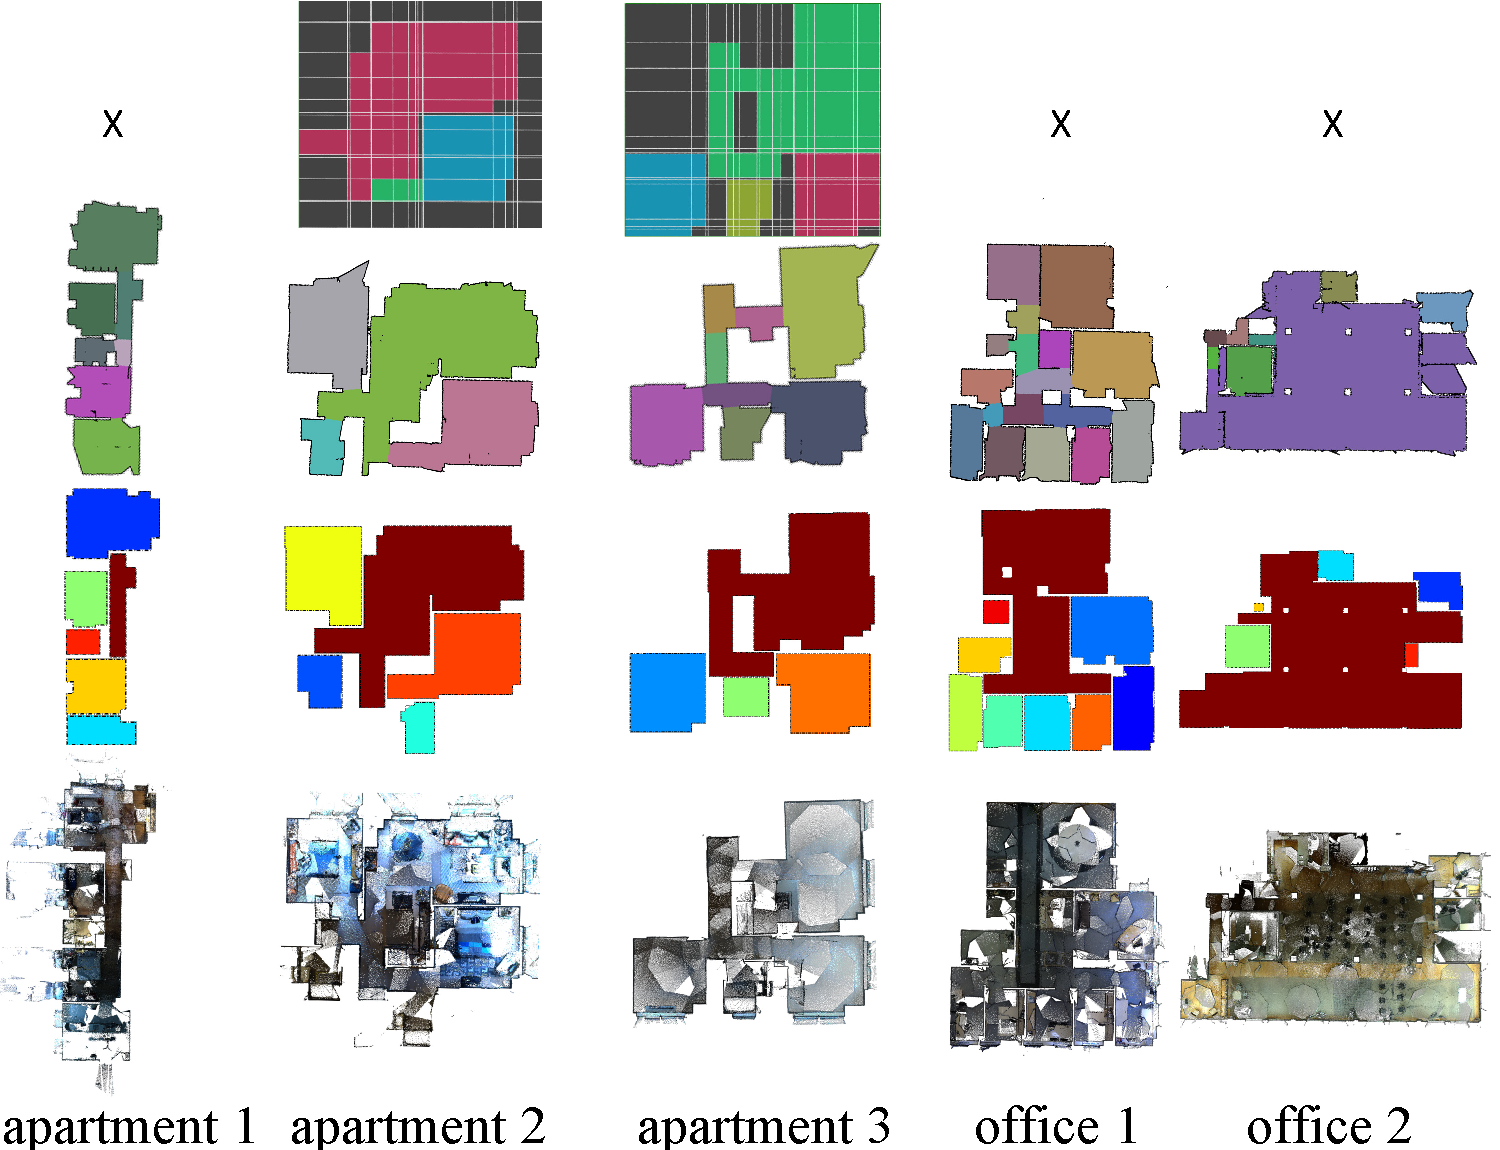
\includegraphics[width=85mm]{../figures/result_all.pdf}
\end{center}
 \vspace{-0.2cm}
\caption{Comparison of the room segmentation algorithms. The first and
second rows are the results by~\cite{Mura2014} and
\cite{Turner2015}, respectively. The third rows contain ours. The bottom
 rows show the input point clouds for reference.}  \label{fig:result_all}
 \vspace{-0.25cm}
\end{figure}



% Finally, we show the experimental results that show our algorithm can
% easily control the complexity of the manifold meshes, which will be
% important for mobile application, where the rendering power varies
% depending on the device but is limited. In this experiment we control
% the complexity of the mesh by three parameters the maximum number of
% meshes about (entire scene, each room, each wall). Then our system
% automatically generate the manifold meshes by cutting off leaf nodes so
% that the constraint is satisfied. We show some examples of the meshes
% in~\Fref{fig:complexity2}.


% \begin{figure}[!t]
% \begin{center}
% 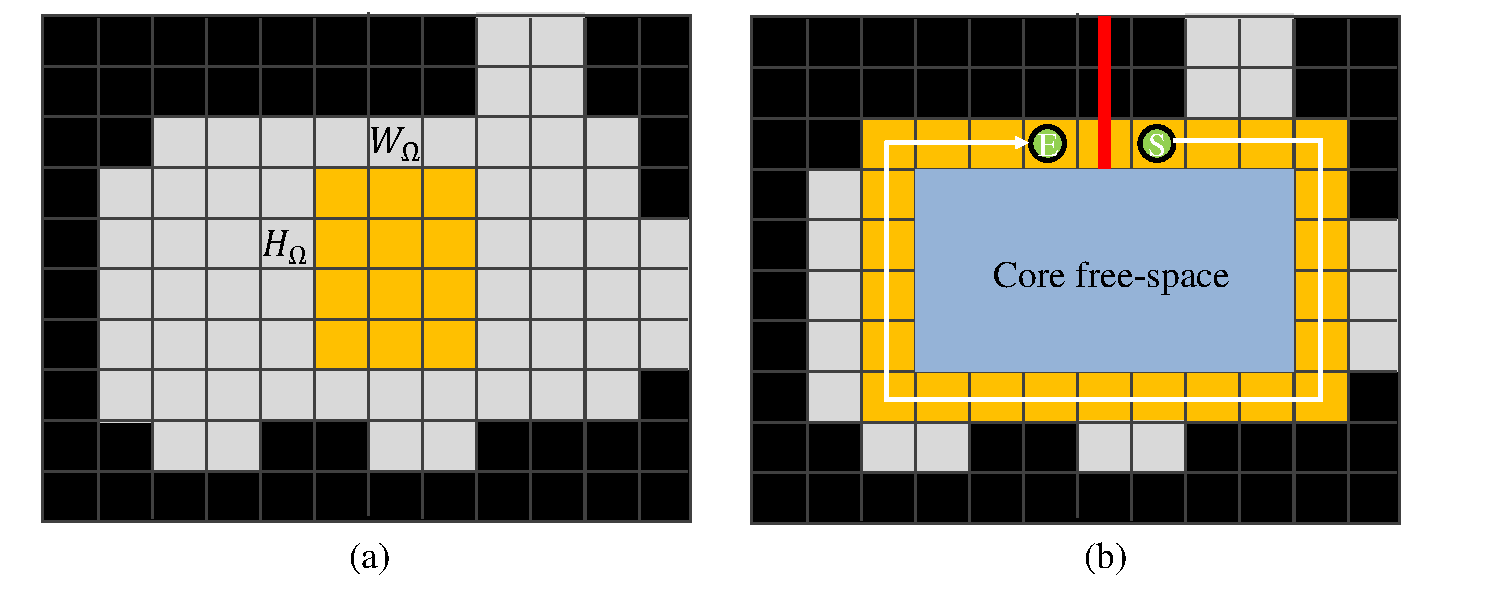
\includegraphics[width=85mm]{../figures/shortestpath.pdf}
% \end{center}
% \caption{Comparison of the surface meshes of the real dataset. Here we show the result of (a) ours, (b) SCPoission, and (c) VGCuts. The same number of polygons are used for each model.}
% \label{fig:shortestpath}
% \end{figure}

%\begin{figure}[!t]
%\begin{center}
%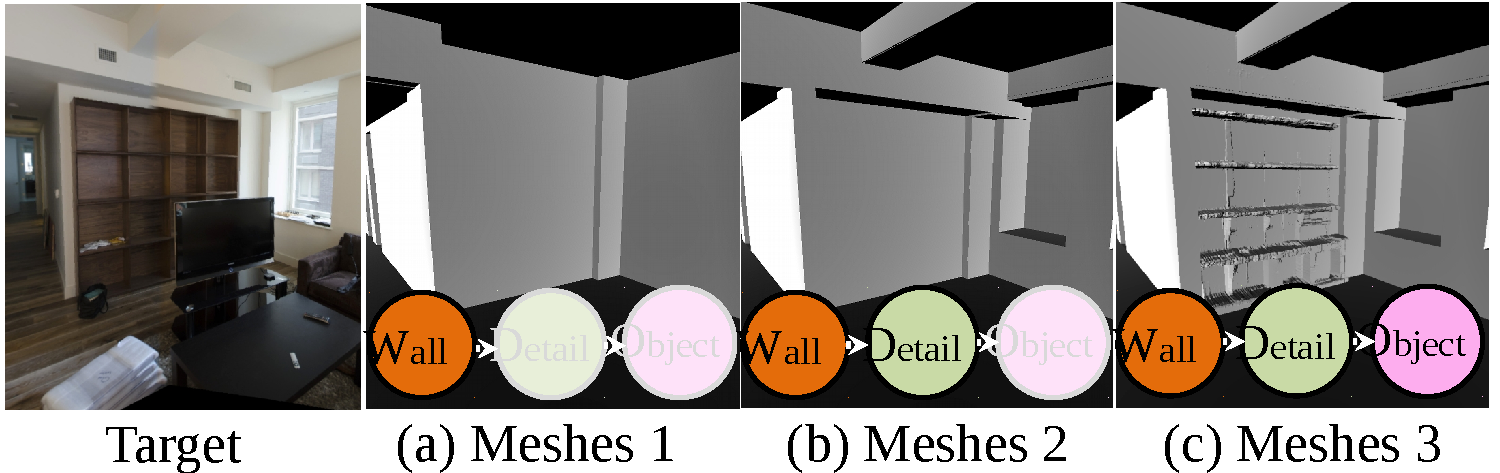
\includegraphics[width=85mm]{../figures/complexity.pdf}
%\end{center}
%\caption{We can compile the manifold meshes from a structured graph by changing the deepest nodes to be compiled. Here we show three examples where (a) wall nodes, (b) wall and their children detail nodes, and (c) wall, detail, and object nodes are compiled.}
%\label{fig:shortestpath}
% \vspace{-0.25cm}
%\end{figure}



%One key distinction in our reconstruction
%algorithms is that we rely on global optimizations to produce compact 3D
%%models without any primitive detection. 


%never extract a geometric primitive, while most
%existing methods for compact 3D reconstruction relies on primitive
%extraction, which is often
%A key design 
%One key design decision in the algorithm selection

